In the work done by Tolle \cite{Tolle00} some dynamical systems were proposed and theye checked if the first digit distribution followed Benford's Law. We took 2 autonomous circuits which displayed chaotic behaivour and verified if they were conformant according with the criterion given by Nigrini et. al. \cite{Nigrini97}. According to our experimental results, the system which best followed the distribution whas the Third Order Autonomous System proposed by Takougang et.al \cite{Takougang13}.

Verifyng the results from \cite{Takougang13}, we notice that this circuit has a Shilnikov heteroclinic orbit, which implies by the Shilnikov Criterion that the system has horseshoe chaos. This type of chaos produces time signals called chaotic bursting oscillations (see Fig. 4.1)
\begin{figure}[h]
            \centering
            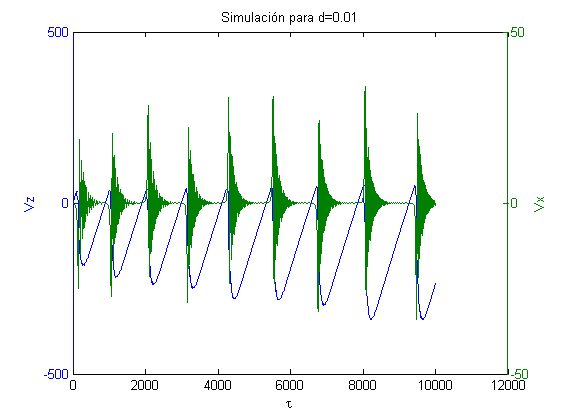
\includegraphics[scale=0.6]{imagenes/2-benford/bursting_oscilatons.png}
            \caption{$V_y$ response as a function of time}
            \end{figure}


This type of oscillations are found in biological phenomena, such as $Ca^2+$ oscillations in non-excitable cells \cite{Perc03}, pancreatic $\beta$ cells \cite{Sherman88} and in neurons\cite{Ermentrout09} and heart oscillatons, also, the work by Kreuzer et. al. \cite{Kreuzer14} indicates that brain electrical activity follows Benford's Law, so it would be interesting to see if Benford's Law could be an indicative if Real life phenomena is modelled correctly by the system if both follow Benford's Law (as it was first indicated by \cite{Tolle00}) and also to try to verify if other systems that present this kind of oscillations also follow Benford's Law.
